\documentclass[12pt]{article}

\usepackage{cawsty}

\title{On the L(2,1) Span of k-Regular t-Partite Graphs}
\author{
        Christopher A. Wood \\
        {\tt woodc1@uci.edu} \\
        % \url{www.christopher-wood.com}
}
\date{\today}

\begin{document}
\maketitle

%%% ABSTRACT
\begin{abstract}
TODO
\end{abstract}

%%%%%%%%%%%%%%%%%%%%%
%%% MAIN CONTENT
%%%%%%%%%%%%%%%%%%%%%

\section{Introduction} \label{sec:introduction}
The channel assignment problem, first introduced by Hale and later modified by Roberts \cite{Calamonery-LhkSurvey}, is a long-standing problem that asks for the assignment of frequencies to transmitters based on their distance to nearby nodes in the same network to avoid interference. Since its inception, it has been formulated in terms of graphs as the $L(h,k)$-labeling problem. An $L(h,k)$-labeling of a graph $G$ is an integer labeling of the vertices such that adjacent vertices differ in label by at least $h$, and vertices that are at distance two from each other differ in label by at least $k$. That is, an \emph{$L(h,k)$-labeling} of $G$ is a vertex labeling $f : V(G) \to \{0\} \cup \mathbb{Z}^+$ such that 
\begin{enumerate}
  \item $|f(u) - f(v)| \geq h$ for all $uv \in E(G)$,
  \item $|f(u) - f(v)| \geq k$ if $d(u,v) = 2$.
\end{enumerate}

In the context of this labeling scheme, we define the \emph{span of an $L(h,k)$-labeling $f$} on a graph $G$ as the maximum $f(u)$ for all $u \in V(G)$. The $L(h,k)$-\emph{span of a graph $G$}, denoted $\lambda_{h,k}(G)$, is the minimum span of all $L(h,k)$-labelings on $G$. An $L(h,k)$-labeling $f$ on $G$ whose span is equal to the span of $G$ is called a \emph{span labeling} of $G$.

In 2005, Fiala and Kratochvíl proved that deciding whether a $k$-regular graph, $k \geq 3$, admits a $L(2,1)$ labeling with span $k + 2$ is NP-complete \cite{Coppo05-1}. Furthermore, this bound is optimal, as it is not possible for a $k$-regular graph to admit a $L(2,1)$ labeling with a span of $k + 1$ \cite{Georges03-1, Calamonery-LhkSurvey}. To our knowledge, tight upper bounds for regular graphs has not been formally studied in the literature. 

The general upper bound for the $L(2,1)$ span of arbitrary graphs $G$, given as $\lambda_{2,1}(G) \leq \Delta^2 + \Delta - 2$ \cite{81 - survey}, the span of bipartite graphs $G$ (i.e. $t$-partite graphs with $t = 2$), is bounded by $\lambda_{2,1}(G) = \Omega(\Delta^2)$. Furthermore, the decisional version of the $L(2,1)$ labeling problem was shown to be NP-complete for planar bipartite graphs in \cite{20 - survey}. The $L(2,1)$ span of $t$-partite graphs for $t > 2$ has also not been studied in the literature. 

In this work we consider $k$-regular $t$-partite graphs $G$. We build on previous results from regular and bipartite graphs to show that $\lambda_{2,1}(G) \{5,6\}$ for bicubic ($k = 3$ and $t = 2$) graphs, and discuss several generalizations to arbitrary non-negative values of $k$ and $t$. 

\section{Bicubic Graphs}
Bicubic graphs are bipartite 3-regular graphs, are a simple structure to study and can be easily generated using the \emph{nauty} \cite{nauty}. The smallest bicubic graph is $K_{3,3}$, shown in Figure \ref{fig:k33}. One may easily determine that $\lambda(K_{3,3}) = 6$. The smallest bicubic graph that admits a $L(2,1)$ span of $5$ is shown in Figure \ref{fig:n12_bicubic}, along with the specific vertex labels that realize this label span. This graph was found computationally by enumerating all bicubic graphs up to 12 vertices using nauty, of which there exists only 9 nonisomorphic graphs, and then exhaustively checking all possible $6^{12} = 2,176,782,336$ vertex labelings that use labels from the set $\{0,1,2,3,4,5,6\}$. 

\begin{figure}
\centering
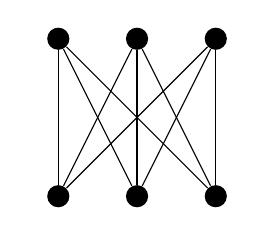
\begin{tikzpicture}[shorten >=1pt,->]
	\tikzstyle{minor}=[circle,fill=black,minimum size=8pt,inner sep=2pt]
	\tikzstyle{vertex}=[circle,fill=black,minimum size=8pt,inner sep=2pt]
	\tikzstyle{major}=[isosceles triangle,shape border rotate=90,fill=black,minimum size=8pt, inner sep=2pt]
	\tikzstyle{top}=[rectangle,fill=black,minimum size=8pt, inner sep=2pt]
	\node[minor, label=left:{}] (V1) at (-1, 1) {};
	\node[minor, label=left:{}] (V2) at (0,1)	 {};
	\node[minor, label=right:{}] (V3) at (1, 1) {};
	\node[minor, label=right:{}] (V4) at (-1,-1)	 {};
	\node[minor, label=left:{}] (V5) at (0,-1) {};
	\node[minor, label=right:{}] (V6) at (1,-1) {};

	\draw (V1) -- (V4) -- cycle;
	\draw (V1) -- (V5) -- cycle;
	\draw (V1) -- (V6) -- cycle;

	\draw (V2) -- (V4) -- cycle;
	\draw (V2) -- (V5) -- cycle;
	\draw (V2) -- (V6) -- cycle;

	\draw (V3) -- (V4) -- cycle;
	\draw (V3) -- (V5) -- cycle;
	\draw (V3) -- (V6) -- cycle;
\end{tikzpicture}
\caption{$K_{3,3}$}
\label{fig:d4n1}
\end{figure}

\begin{figure}
\centering
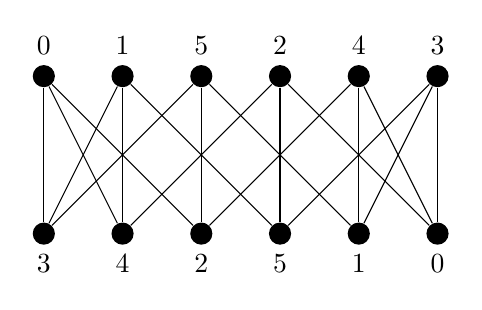
\begin{tikzpicture}[shorten >=1pt,->]
	\tikzstyle{minor}=[circle,fill=black,minimum size=8pt,inner sep=2pt]
	\tikzstyle{vertex}=[circle,fill=black,minimum size=8pt,inner sep=2pt]
	\tikzstyle{major}=[isosceles triangle,shape border rotate=90,fill=black,minimum size=8pt, inner sep=2pt]
	\tikzstyle{top}=[rectangle,fill=black,minimum size=8pt, inner sep=2pt]
	\node[minor, label=above:{$0$}] (V1) at (-2, 1) {};
	\node[minor, label=above:{$1$}] (V2) at (-1,1)	 {};
	\node[minor, label=above:{$5$}] (V3) at (0, 1) {};
	\node[minor, label=above:{$2$}] (V4) at (1,1) {};
	\node[minor, label=above:{$4$}] (V5) at (2,1) {};
	\node[minor, label=above:{$3$}] (V6) at (3,1) {};
	\node[minor, label=below:{$3$}] (V7) at (-2, -1) {};
	\node[minor, label=below:{$4$}] (V8) at (-1,-1) {};
	\node[minor, label=below:{$2$}] (V9) at (0, -1) {};
	\node[minor, label=below:{$5$}] (V10) at (1,-1) {};
	\node[minor, label=below:{$1$}] (V11) at (2,-1) {};
	\node[minor, label=below:{$0$}] (V12) at (3,-1) {};

	% K??FEagT@WB_,5,{0=0, 1=1, 2=5, 3=2, 4=4, 5=3, 6=3, 7=4, 8=2, 9=5, 10=1, 11=0}

	\draw (V1) -- (V7) -- cycle;
	\draw (V1) -- (V8) -- cycle;
	\draw (V1) -- (V9) -- cycle;

	\draw (V2) -- (V7) -- cycle;
	\draw (V2) -- (V8) -- cycle;
	\draw (V2) -- (V10) -- cycle;

	\draw (V3) -- (V7) -- cycle;
	\draw (V3) -- (V9) -- cycle;
	\draw (V3) -- (V11) -- cycle;

	\draw (V4) -- (V8) -- cycle;
	\draw (V4) -- (V10) -- cycle;
	\draw (V4) -- (V12) -- cycle;

	\draw (V5) -- (V9) -- cycle;
	\draw (V5) -- (V11) -- cycle;
	\draw (V5) -- (V12) -- cycle;

	\draw (V6) -- (V10) -- cycle;
	\draw (V6) -- (V11) -- cycle;
	\draw (V6) -- (V12) -- cycle;
\end{tikzpicture}
\caption{The smallest order bicubic graph $G$ such that $\lambda_{2,1}(G) = 5$.}
\label{fig:n12_bicubic}
\end{figure}

We then tried this same exhaustive computation procedure for graphs of larger order $n = 16$ and $n = 16$, of which there exists $35$ nonisomorphic candidates. In doing so, we found that in no case did the smallest possible label span exceed $6$, which inspired the following theorem. 

\begin{thm}
$\lambda_{2,1}(G) \in \{5,6\}$ for any bicubic graph $G$. 
\end{thm}
\begin{proof}
Based on the results of Georges et al. \cite{Georges03} and the label span presented for the graph in Figure \ref{fig:n12_bicubic}, we know that $5$ is the smallest possible label that may be admitted for bicubic graphs. Furthermore, if $S$ and $T$ represent the two vertex partite sets of a bicubic graph $G$, then without loss of generality it is clear that a minimal $L(2,1)$ labeling will label vertices from $S$ with labels from one set $\{0,1,\dots,m-1\}$ and vertices from $T$ with labels from distinct set $\{m+1,m+2,\dots,\lambda_{2,1}(G)\}$. 

To prove that $6$ is the largest label required for a minimal $L(2,1)$ span, assume that there exists a graph $G$ such that $\lambda_{2,1}(G) = 7$. This means that there must be some critical vertex $v_c$ such that $f(v_c) = 7$. Assume, for the sake of contradiction, that $v_c$ cannot be labeled from the set $\{0,1,\dots,5,6\}$. Consider the vertices in the $S$ set. We first claim that for all $v \in S$ it is true that $f(v) \in \{0,1,2\}$. To show this, assume, without loss of generality, that there exists some vertex $u \in S$ such that $f(u) = 3 > 2$. Since $u$ is at distance at least $2$ from every other vertex in $S$, the only condition that would force $f(u_i) = 4$ is that there exists three vertices $u_j$, $u_k$, and $u_l$ such that
\begin{align*} 
d(u_i,d_j) = d(u_i, u_k) = d(u_i,u_l) = d(u_j,u_k) = d(u_j,u_l) = d(u_k,u_l) = 2,
\end{align*}
and, without loss of generality, $f(u_j) = 0$, $f(u_k) = 1$, and $f(u_l) = 2$. This implies that there exists another vertex $v \in T$ that is adjacent to $u_i$, $u_j$, $u_k$, and $u_l$. Since $G$ is 3-regular, such a vertex $v$ cannot exist. Therefore, there must exist at least one vertex in the set $\{u_j,u_k,u_l\}$ that is not at distance $2$ from $u_i$. Without loss of generality, let $u_j$ be this vertex. Since $d(u_i,u_j) > 2$, we can therefore let $f(u_i) = f(u_j) = 0$. The same holds true for any vertex in $S$.

Since the labels of all vertices in $S$ is upper bounded by $2$, and every vertex in $S$ is adjacent to a vertex in $T$, we assume that labeling vertices in $T$ will start at $4$. Again, we claim that for all $v \in T$ it is true that $f(v) \in \{4,5,6\}$. Using a similar argument as for the vertices of $S$, one can easily show that this is true. Therefore, the label of $v_c$ is not forced to $7$, and we have a contradiction.

% TODO: maybe it would be better to show that 0,1,2 is all that's needed for the lower partite set (4 isn't needed because of the argument in my notes), and that means that 4 will be the smallest label for upper partite set, and therefore it isn't possible to force a label to 7 because the labels need only be 4,5,6 (i.e. if we assume there's one with a label of 7 then it must be 2-adjacent to vertices with 4,5,6, which can't happen if 3-regular, and therefore 7 can be 2-adjacent to either 4-5, 4-6, or 5-6, and all cases it can just assume the missing label of 6, 5, or 4). Done!

\end{proof}

\begin{cor}
$\lambda_{2,1}(G) \in \{k + 2,\dots, 2k\}$ for any $k$-regular bipartite graph $G$. 
\end{cor}
\begin{proof}
Using a similar argument as in the bicubic case, we can show that it is always possible to label $G$ from the set $\{k + 2,\dots, 2k\}$. The proof follows the same structure with the only difference being that we assume the vertices in the lower partite set $S$ can always be assigned labels from the set $\{0,1,\dots,m - 1\}$, and the vertices in the upper partite set $T$ can always be assigned labels from the set $\{m + 1,\dots,2k\}$. 
\end{proof}

\section{Generalizations to $k$-regular $t$-partite graphs}

After generalizing the $L(2,1)$-span for $k$-regular bipartite graphs, it is natural to ask if we can also extend the results to any $k$-regular $t$-partite graph, $k,t > 2$. By again applying our ``tower'' approach to labeling the $t$ partite sets of a $t$-partite $k$-regular graph $G$, we obtain the loose bounds.

\todo[inline]{I need to formalize what I mean by this tower approach to labeling the partite sets, but I think it's clear from context.}

\begin{cor}
$\lambda_{2,1}(G) \in \{k+2,\dots,(tk + t + k - 1)\}$ for any $t$-partite $k$-regular graph $G$. 
\end{cor}
\begin{proof}
The lower bound is again a trivial realization of Georges et al. \cite{Georges03} in that $\lambda_{2,1}(G) > k+1$. The upper bound is established in the following way. Let $S_1,S_2,\dots,S_t$ denote the $t$ partite sets of the graph $G$. Using the tower labeling approach, we know that the vertices in $S_1$ can receive labels from the set $\{0,1,\dots,k-1\}$. Now, by enforcing that $f(v_i) \not= k$ for all $v_i \in V(G)$ (i.e. by skipping a label in the sequence from $0,1,\dots,(tk + t + k - 1)$), the vertices in $S_2$ can be labeled with the next $k$ smallest labels, namely, $\{k+1,k+2,\dots,2k\}$. By following this sequence of label skipping and tower assignment, we obtain the following recurrence relation that defines the minimum label $l_i$ for a partite set $S_i$ given $i$:
\begin{align*}
l_1 & = 0 \\
l_i & = (k + 1) + l_{i-1} 
\end{align*}
Solving this recurrence relation for $i = t$ yields $l_t = t(k + 1)$. Since this last partite set will have $k$ distinct labels by our above arguments, and $l_t$ will be included in this label set, we therefore know that the upper bound will be $l_t + (k - 1)$, or simply, $tk + t + k - 1$.
\end{proof}

For large values of $t$ and $k$, this upper bound is quite loose. We therefore took a computational approach to determine if indeed we can always find smaller $L(2,1)$-spans for these graphs. This computational approach can be summarized as follows:
\begin{enumerate}
	\item Exhaustively generate all $k$-regular $t$-partite graphs with order $n$ up to feasible values of $n$.
	\item Run the exhaustive $L(2,1)$ labeling program on each of these graphs to determine a minimum span.
\end{enumerate}
Clearly, both tasks are computationally expensive. To the best of our knowledge there does not exist an efficient algorithm for generating $t$-partite graphs. However, Meringer \ref{Meringer1999-1} devised an efficient algorithm for generating regular graphs that has been used by the community to generate a fairly exhaustive list of regular graphs for sufficiently large values of $n$. These results are summarized in Table \ref{tab:reg-graphs}.

\begin{table}
\centering
\caption{Number of regular $k$-regular graphs for various values of $n$.}
\caption{tab:reg-graphs}

\begin{tabular}{|c|} \hline
$k$ \\
% TODO: insert table here...
\end{tabular}

\end{table}

Using the program {\tt reggen}, which is an open-source implementation of the regular graph generation algorithm developed by Meringer, we then used SAGE to find the chromatic number for each of these graphs, as this tells us whether or not the graph $G$ is $\chi(G)$-partite. Finally, after properly categorizing this exhaustive set of $k$-regular $t$-partite graphs, we then ran our $L(2,1)$ labelling program on all $TOTAL$ graphs. 

\todo[inline]{Need to cite reggen, SAGE, and webpage with the table of graphs}
\todo[inline]{Need to figure out if there's a way to run the parallel program on the grid... Or, maybe, GPU? See Kaminsky's GPU code for examples}

%%%%%%%%%%%%%%%%%%%%%
%%% END MAIN CONTENT
%%%%%%%%%%%%%%%%%%%%%

%%% BIBLIOGRAPHY
\bibliographystyle{abbrv}
\bibliography{OTLSOKTG_Wood_2013}

\end{document}
